%%%% CAPÍTULO 3 - MATERIAL E MÉTODOS (PODE SER OUTRO TÍTULO DE ACORDO COM O TRABALHO REALIZADO)

\chapter{Metodologia}\label{cap:metodologia}

Neste capitulo será exposto quais os métodos e materiais utilizados na construção deste trabalho, desde o levantamento da oportunidade de melhoria e do estado da arte, realizados na revisão da literatura, a proposta, o desenvolvimento e a validação de uma solução para os desafios levantados por este trabalho.

\section{Visão Geral}\label{sec:visaogeral}

As etapas de desenvolvimento do Padrão de Rótulos e Interfaces para Sistemas Médicos (PRISM) foram inicialmente definidas de acordo com o demostrado pela Figura \ref{fig:metodologiaGeral}. Após a revisão da literatura sobre o assunto, foram definidos quais requisitos e tecnologias são esperados de uma solução como a apresentada neste trabalho. Posteriormente a definição inicial, o autor escopa os processos que descrevem como os componentes participantes do sistema vão interagir entre si e quais as estruturas de dados obrigatórias para essa interação. Em seguida, inicia-se a construção do Nó de Pesquisa Interoperável (NPI) que servirá como meio de interoperabilidade e espinha dorsal da proposta. 

Finalizada a construção do NPI, o trabalho irá prosseguir com a construção de um projeto exemplo constituído por um sistema de gestão de acesso e voluntários integrado a um sistema de captura de sEMG orquestrado pelo PRISM, onde o armazenamento de dados produzidos pela solução e a gestão de acesso as informações serão feitas por um NPI. Com o projeto exemplo pronto para uso, será populado com dados e biossinais coletados de voluntários, para então validar os resultados obtidos.

\begin{figure}[htb]%% Ambiente figure
    %\captionsetup{width=0.55\textwidth}%% Largura da legenda
    \caption{Fluxograma da visão geral do trabalho}%% Legenda
    \label{fig:metodologiaGeral}%% Rótulo
    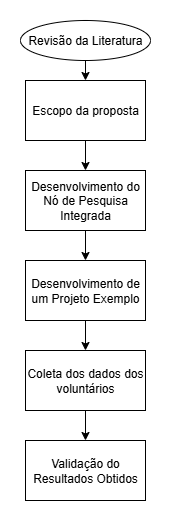
\includegraphics[scale=0.5]{figuras/metodologia/Metodologia.png}%% Dimensões e localização
    \fonte{Autoria própria (2025)}%% Fonte
\end{figure}

\section{Modelo proposto}\label{sec:modeloProposto}

O PRISM busca resolver o problema propondo um modelo de organização para projetos de pesquisa de captura de biossinais, agrupando elementos de um projeto em supernós com funcionalidades específicas, permitindo a visualização e explicitando as principais trocas de informação dos componentes dos projetos de forma normalizada ao reduzir todo o projeto de pesquisa em elementos básicos, o \textit{dispositivo} e a \textit{aplicação}. Essa redução agrupa os componentes do projeto de acordo com suas funcionalidades principais buscando unir os fluxo de dados e seus participantes afim de evidenciar os principais pontos de integração que podem ser interligados a um NPÌ.

Além disso, o PRISM obriga os projetos participantes a ter pelo menos um sistema que possua uma interface em conformidade com os requisitos de estrutura do padrão, incentivando que esse projetos sejam capazes de fazer a conversão de seus dados internos e armazenem seus dados em conformidade aos padrões propostos pelo trabalho, promovendo um consenso entre os projetos que adotem o padrão.

O \textit{dispositivo} é um sistema construído com componentes de hardware e software especializados na captura e transmissão de registros de biossinais originados de seres vivos, ou seja, são sistemas embarcados especialistas em aquisição e transmissão de registros via sensores elétricos, mecânicos, ópticos e químicos que possuem limitações de recursos de memória e processamento. Eles obrigatoriamente entram em contato com o paciente de forma direta ou indireta, através de fluídos, e é operado pelo profissional através da aplicação. São representados por losangos nos diagramas.

A \textit{aplicação} é um sistema construído com componentes de hardware e software generalistas que responsáveis pela adição de contexto, processamento e persistência de longo prazo dos registros enviados pelos dispositivos. Ou seja, computadores pessoais, servidores e dispositivos móveis que rodam um ou mais sistemas com interface gráfica que permitem operar os dispositivos e manipular as informações capturadas a partir deles pelos profissionais de saúde. São representados por círculos no diagrama

O \textit{projeto} é um agrupamento de dispositivos e aplicações que se comunicam entre si com a função de capturar dados biomédicos e construir com contextos específicos com esses dados de acordo com seu objetivo. Ele assume o papel de entidade geradora de dados médicos contextualizados e é um produto da colaboração entre paciente, profissional de saúde, dispositivo e aplicação que é capaz de produzir dados com grande quantidade de rótulos e contexto agregados.

O componente central do PRISM é o \textit{Nó de Pesquisa Interoperável} (NPI), se trata de sistema que gerencia a autenticação, o armazenamento, a validação e o acesso aos dados requerido pelo PRISM para promover o compartilhamento dos dados e uso dos entre aplicações de projetos e outros NPIs, agindo  como um nó moderador da rede.

As figuras \ref{fig:projetoBase}, \ref{fig:identificacao} e \ref{fig:reducaoPrism} mostram o processo de redução do PRISM aplicado a um projeto um sistema de captura de biossinais de sEMG.

\begin{figure}[htb]
    \caption{Diagrama base do projeto}
	\label{fig:projetoBase}
    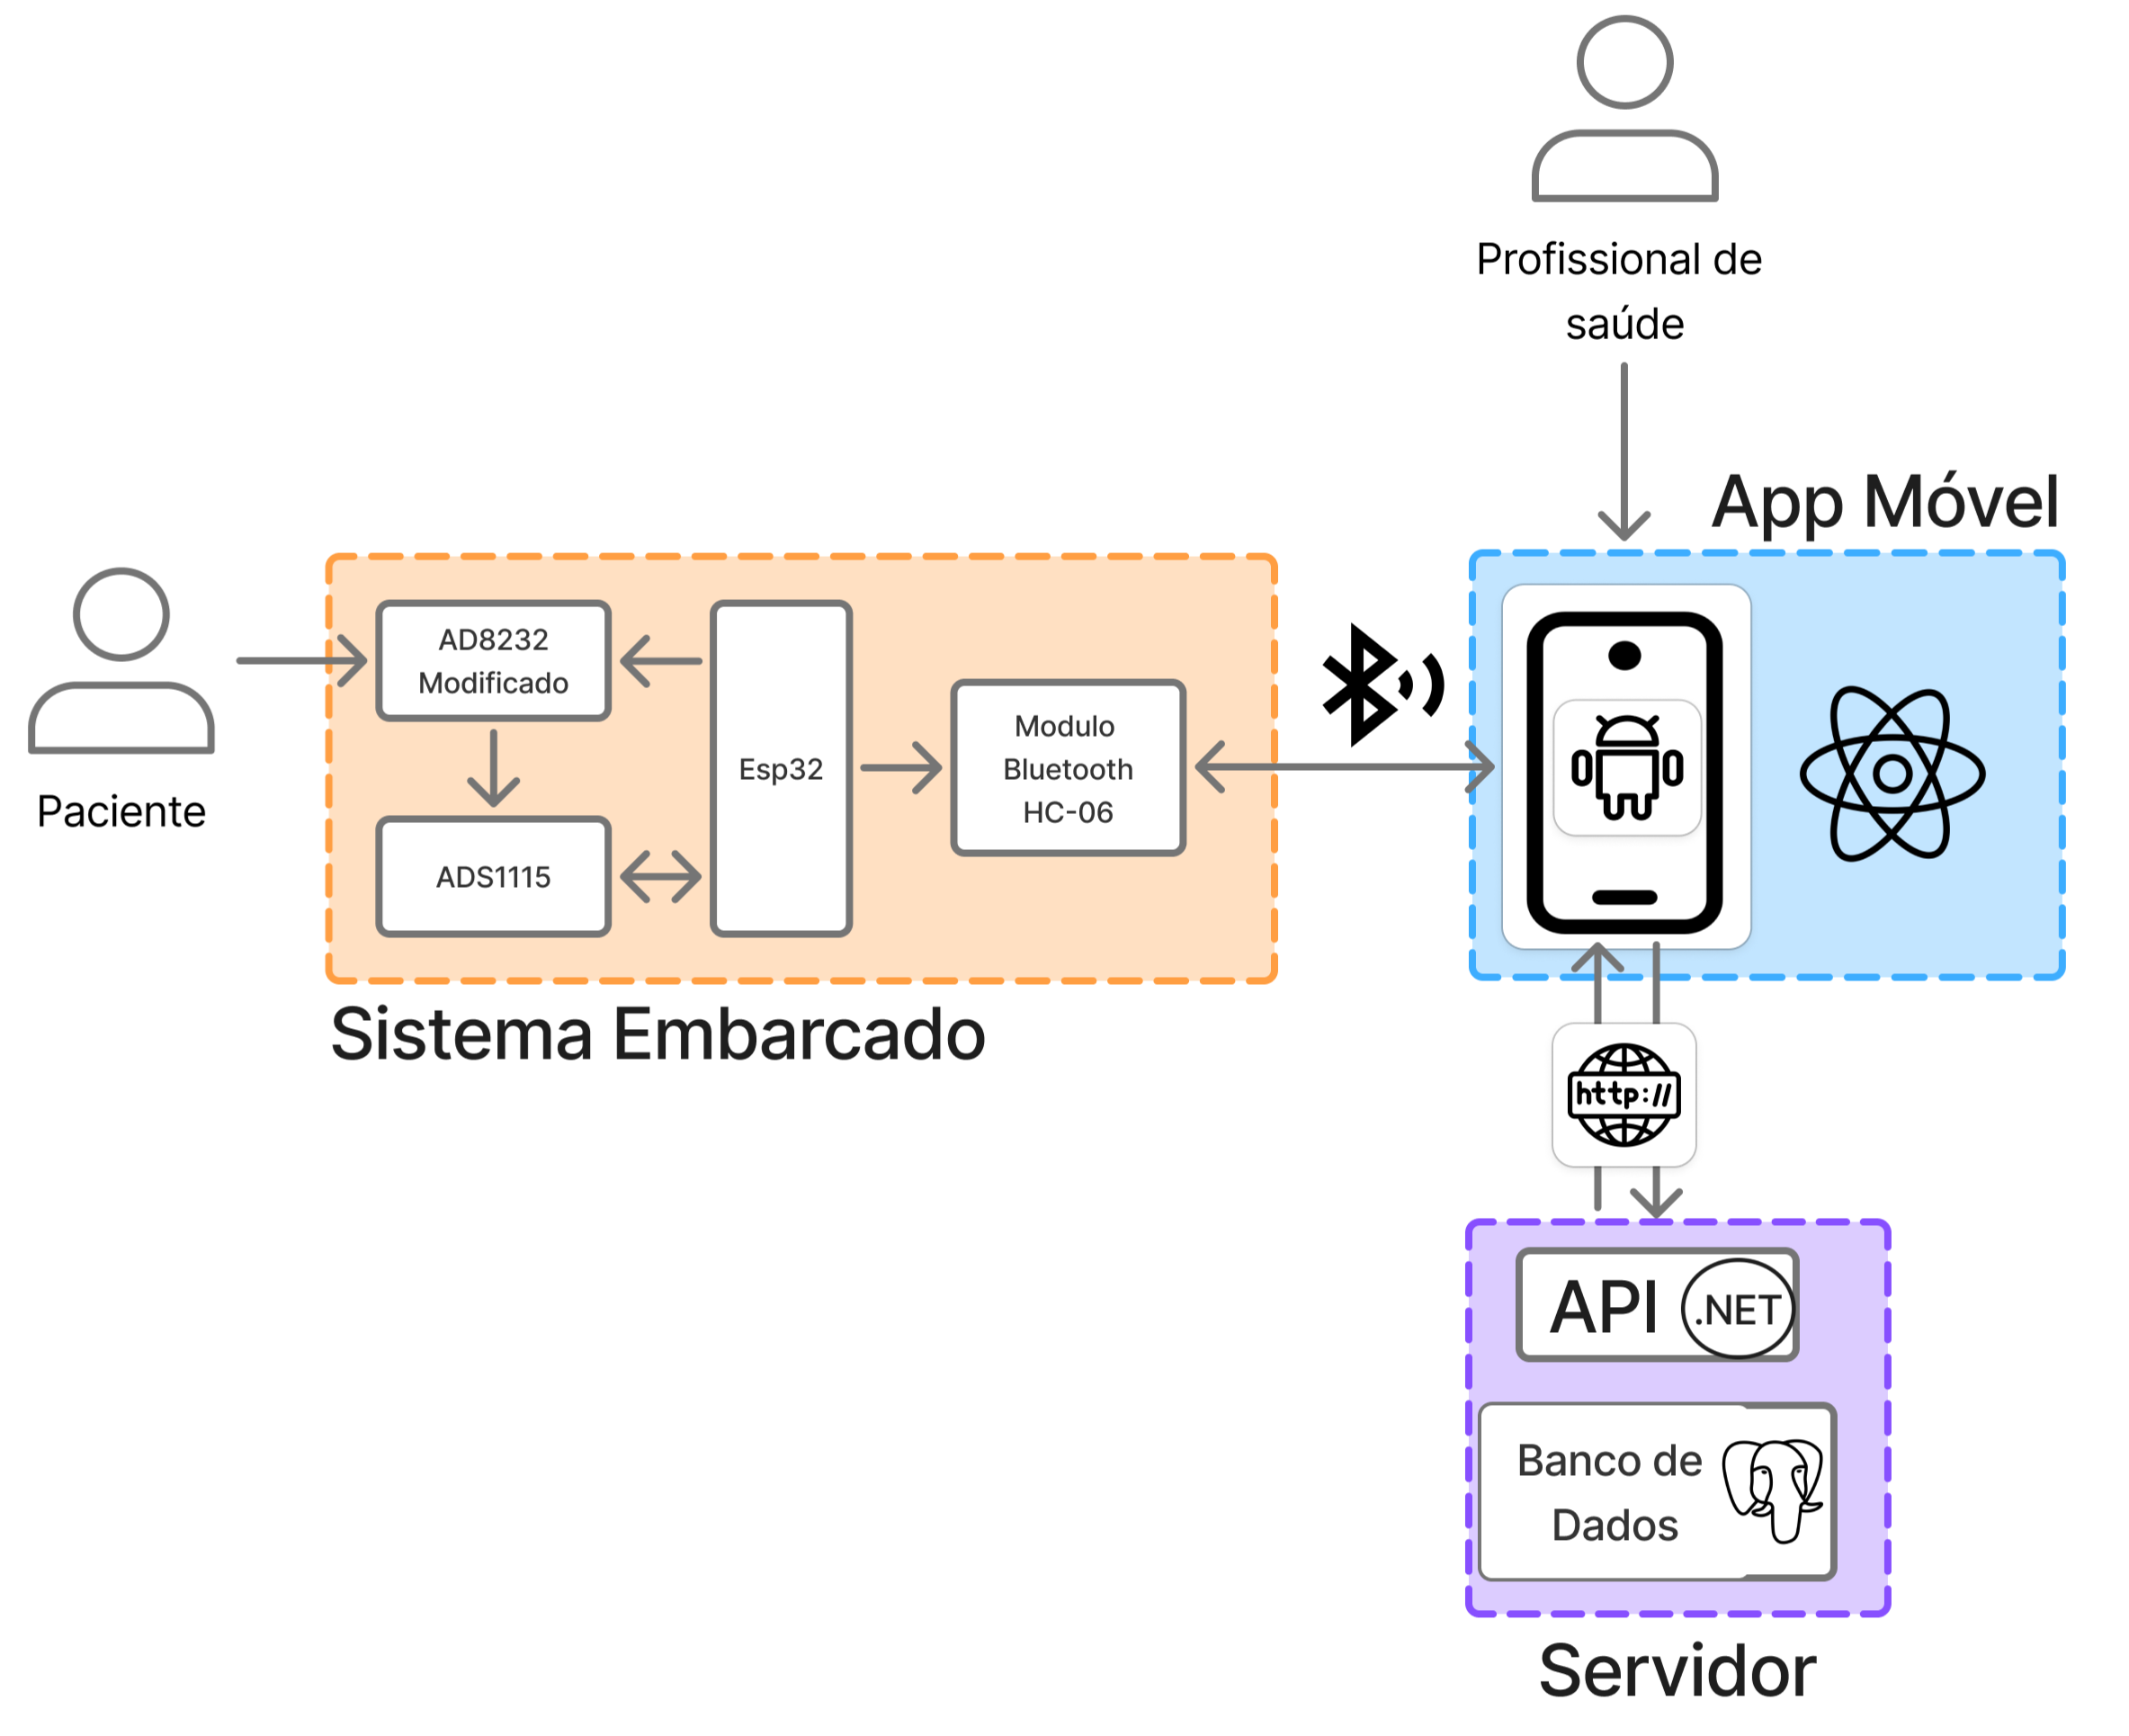
\includegraphics[scale=0.2]{figuras/metodologia/pre-adaptacao.png}%% Dimensões e 
	\fonte{Autoria própria (2025)}
\end{figure}

\begin{figure}[htb]
    \caption{Identificação dos componentes de acordo com o PRISM}
	\label{fig:identificacao}
    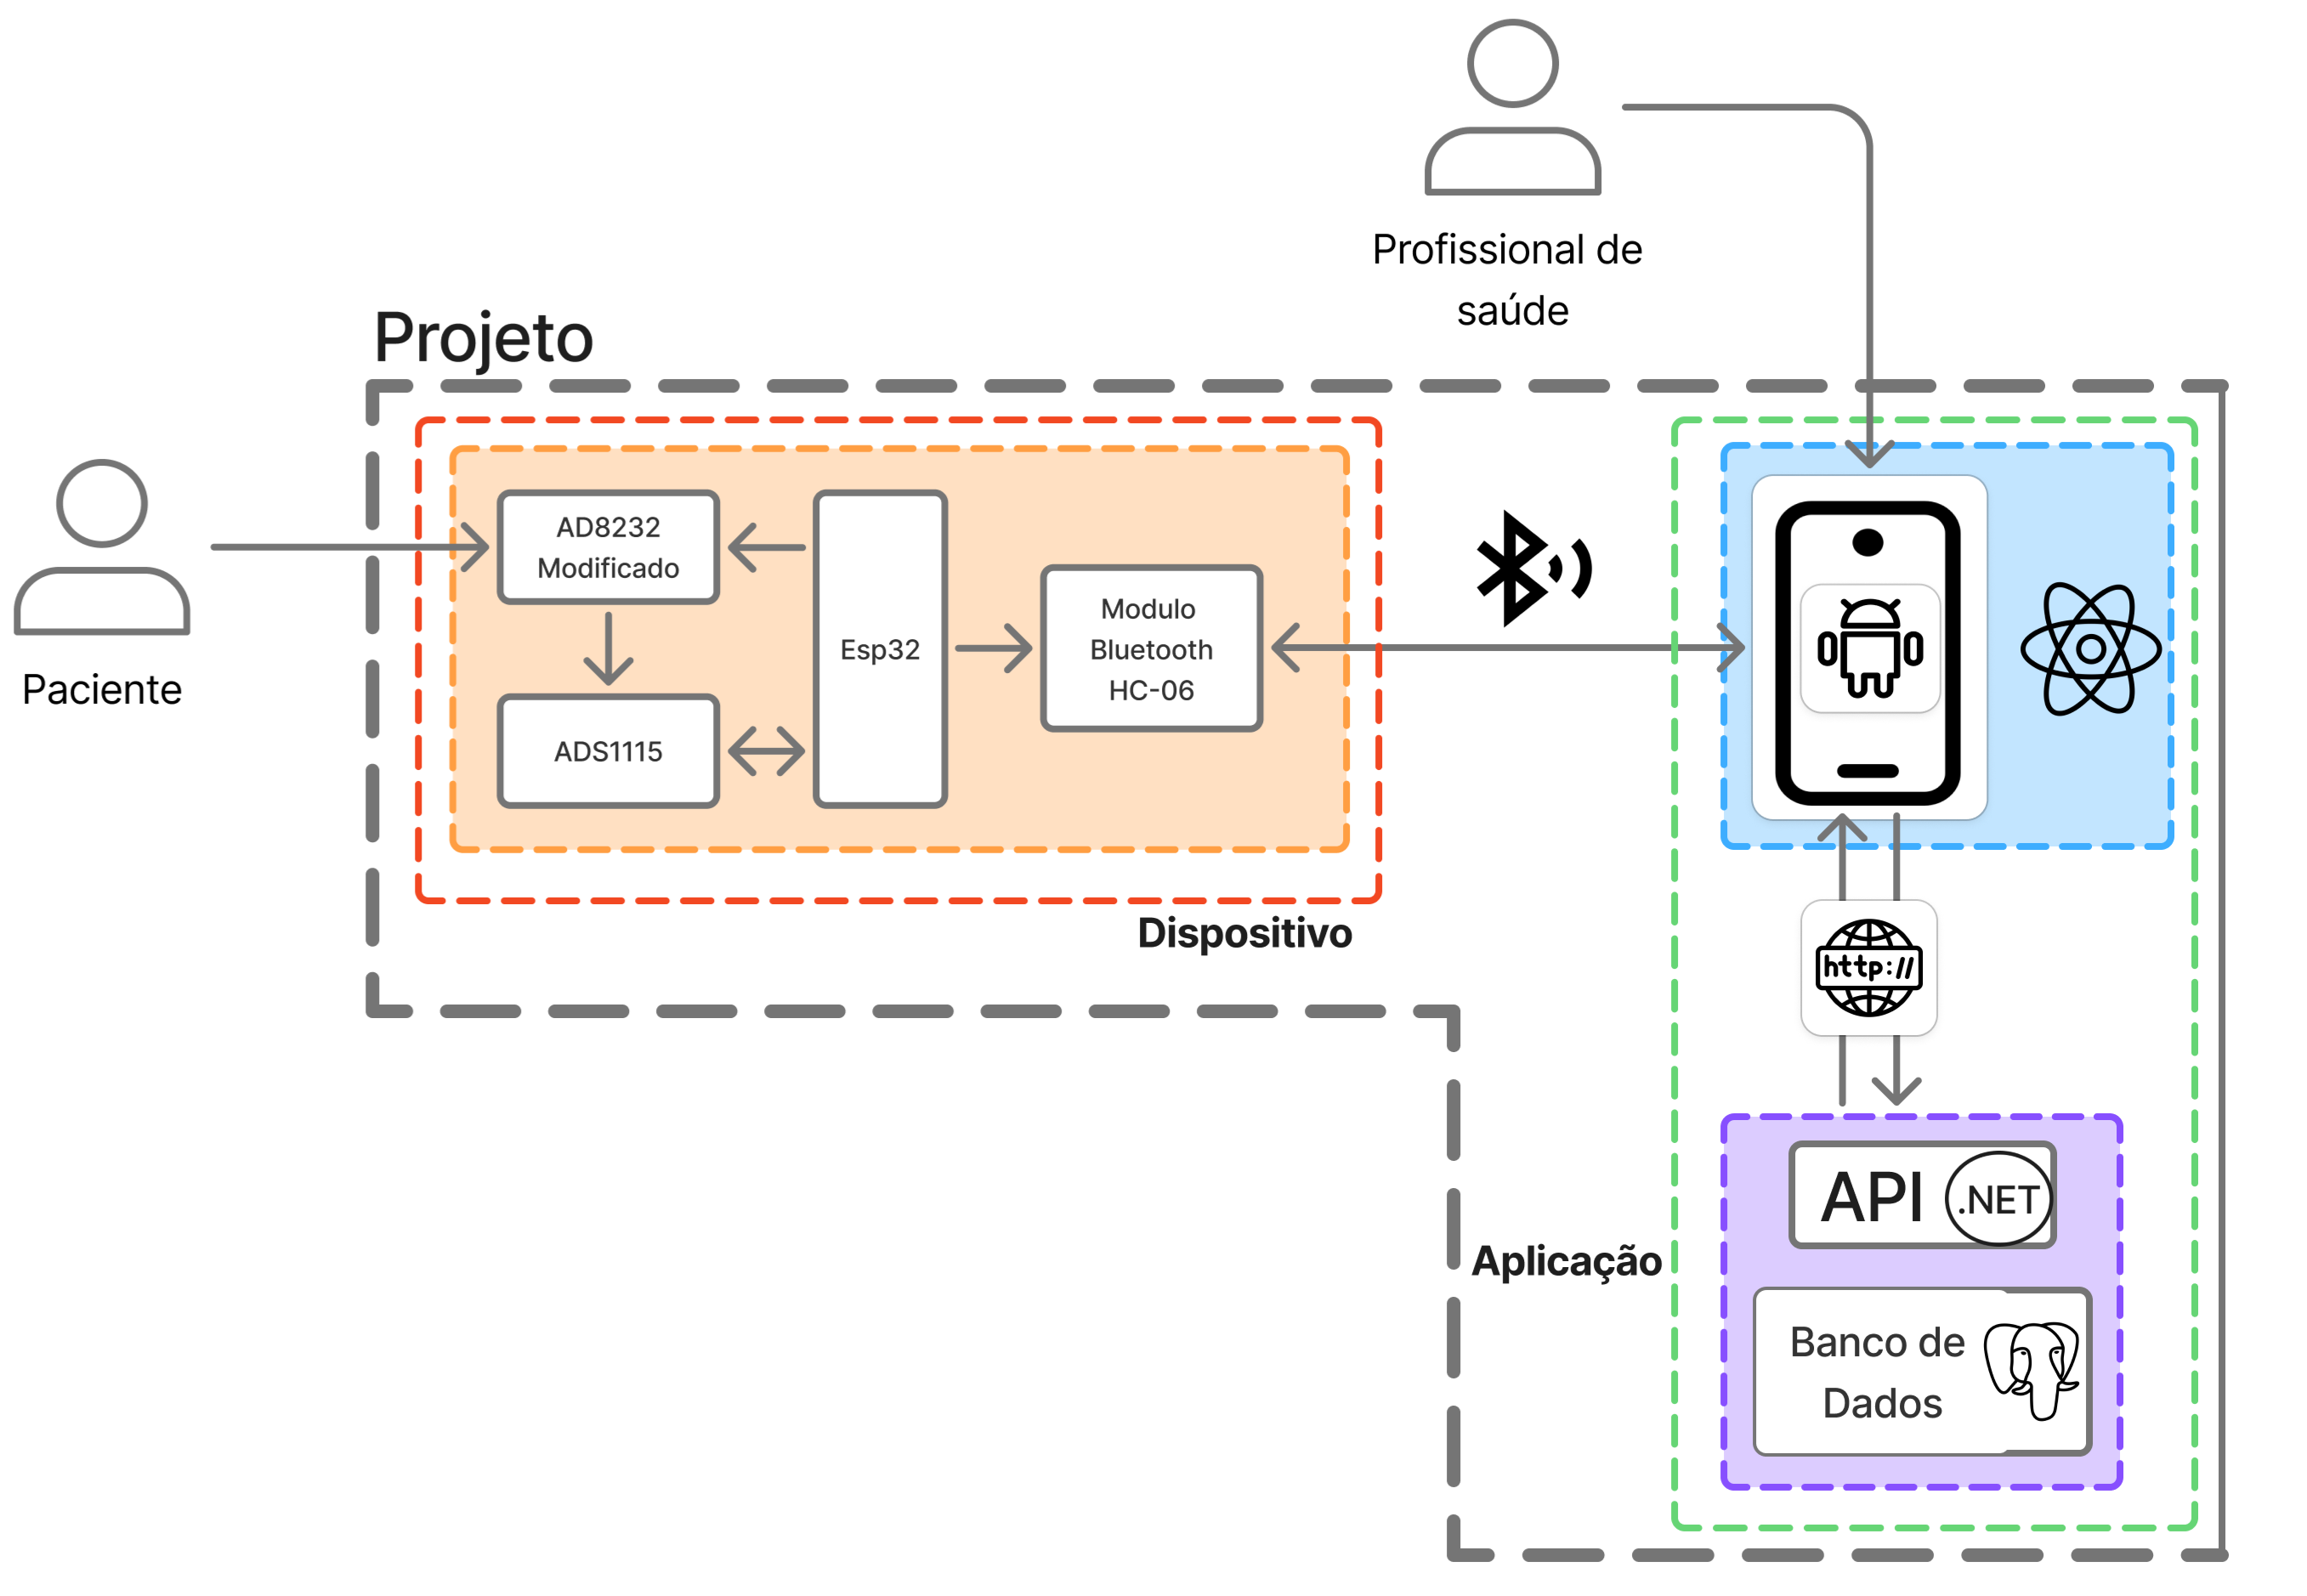
\includegraphics[scale=0.15]{figuras/metodologia/identificacao.png}%% Dimensões e 
	\fonte{Autoria própria (2025)}
\end{figure}

\begin{figure}[htb]
    \caption{Representação do projeto após redução ao PRISM}
	\label{fig:reducaoPrism}
    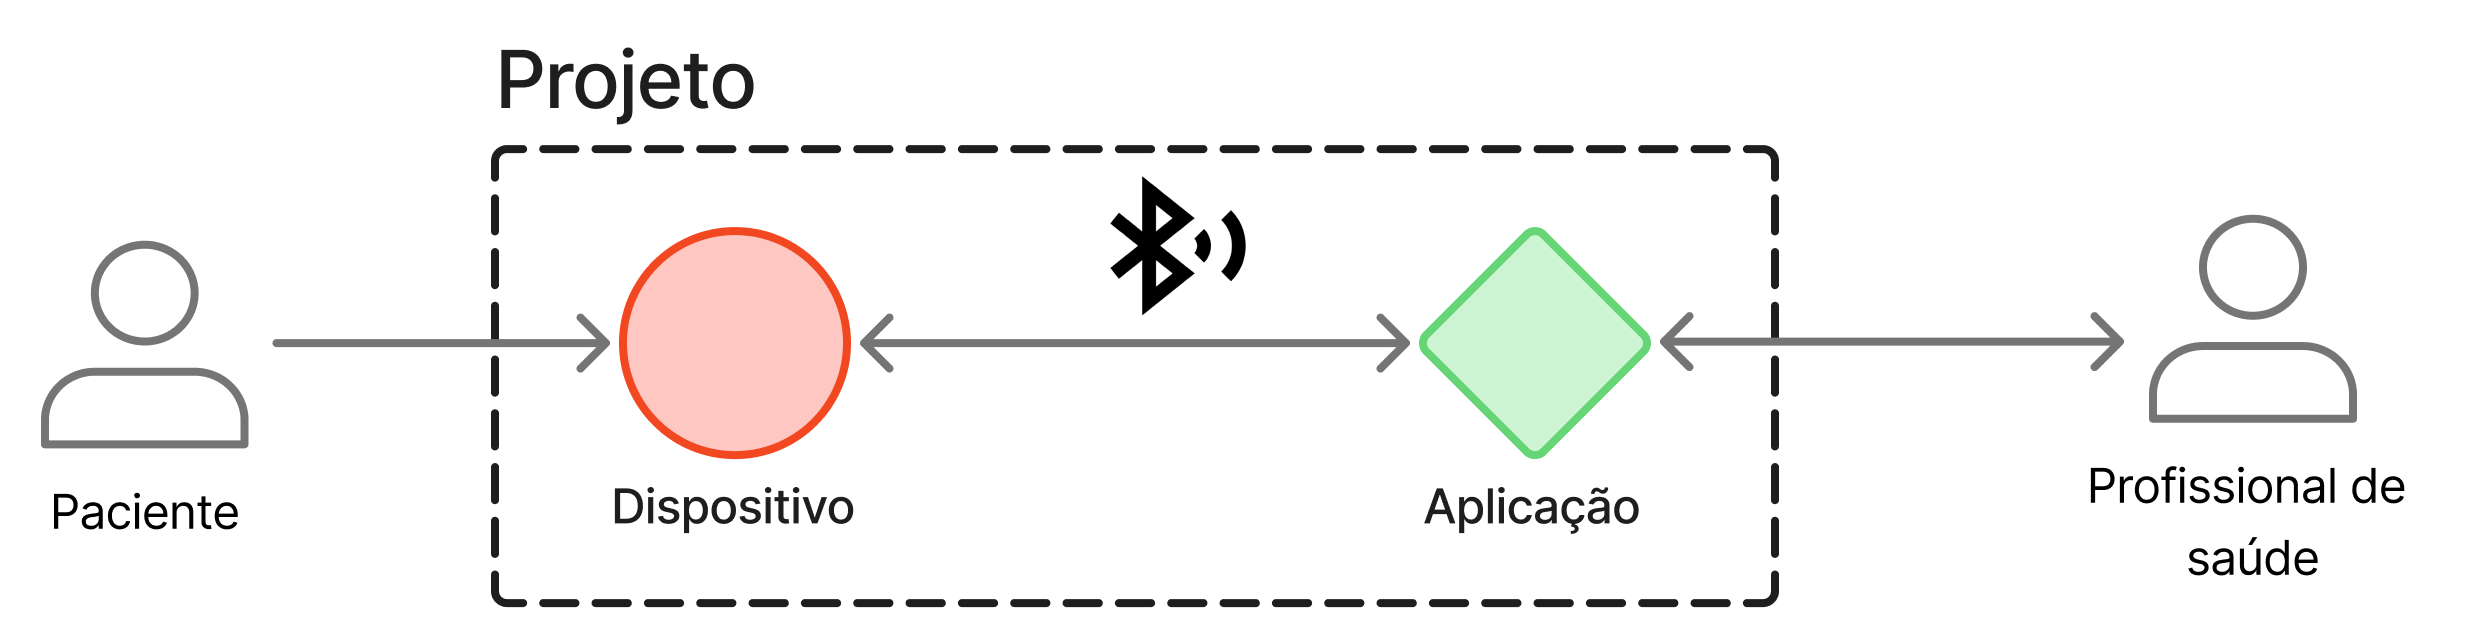
\includegraphics[scale=0.25]{figuras/metodologia/convertido.png}%% Dimensões e 
	\fonte{Autoria própria (2025)}
\end{figure}

\section{Coleta de dados}\label{sec:coletaDeDados}

Esta seção descreve sobre os materiais e métodos utilizados para a coleta de sinais de sEMG dos indivíduos voluntários.

\subsection{NeuroEstimulator}

O NeuroEstimulator é um dispositivo de eletroestimulação funcional (\textit{Functional Electrical Stimulation} — FES) que usa como gatilho a ativação muscular detectada pelo seu sensor de sEMG. O dispositivo possui como microcontrolador o ESP32, utilizando um módulo 8232 para captura e tratamento do sinal de sEMG para ser quantizado pelo módulo conversor analógico digital ADS1115 com capacidade de gerar 860 amostras por segundo. O dispositivo possui um módulo de Bluetooth Classic HC-06 para receber e enviar mensagens utilizando um protocolo de mensagens próprio. O software. O dispositivo é uma versão implementada a partir do trabalho desenvolvido por \cite{veroFES}. O módulo 8232 é uma versão modificada baseada no trabalho de \cite{jjj8232}.

Para este trabalho, foram utilizados apenas os módulos responsáveis pela parte de captura de sEMG, descartando totalmente qualquer utilidade relacionada a estimulação de pacientes

\section{Ferramentas Utilizadas}\label{sec:ferramentas}

Para o desenvolvimento e adaptação das aplicações relacionadas ao NPI e o projeto exemplo, foram usadas as linguagens \textit{C\#} e \textit{Typescript} utilizando as plataformas \textit{Visual Studio 2022} e \textit{Visual Studio Code}. Os dados foram persistidos usando o \textit{PostgreSQL} como banco de dados relacional, \textit{Redis} para registros temporários de cache e o \textit{Azurite} como servidor de arquivos. A infraestrutura resultante foi publicada na forma de contêineres \textit{Docker} em uma máquina virtual hospedada na nuvem \textit{Microsoft Azure}.

 